\section{Biologische Grundlagen}
\label{biologie}
\thispagestyle{plain}

Das visuelle System gehört zu den am gründlichsten untersuchten
Sinnessystemen der Großhirnrinde.  Das liegt nur zum einen an der gut
zugänglichen Lage der Cortexareale, die für die erste visuelle
Reizverarbeitung zuständig sind.  Sie befinden sich bei Säugern direkt
unterhalb der Schädeldecke im hinteren Pol des Großhirns.  Zum anderen
kann man das visuelle System einfach und unter kontrollierten,
reproduzierbaren Bedingungen über die Augen reizen. Es ist sozusagen das
``Wasserstoff--Atom der Hirnforschung''; theoretische Konzepte und
Erklärungsmodelle lassen sich im Experiment am visuellen System
falsifizieren, bzw. können im Wechselspiel mit dem Experiment verfeinert
werden.

In den folgenden Abschnitten werden die für das weitere Verständnis der
Arbeit benötigten biologischen Zusammenhänge, sowie die in dieser Arbeit
behandelten Phänomene erläutert. Der letzte Abschnitt dieses Kapitels
geht dabei auf Ergebnisse einer Datenanalyse ein, bei der in Zusammenarbeit
mit Siegrid Löwel vom Max--Planck--Institut für Hirnforschung die
geometrische Beziehung zwischen Okulardominanz-- und Orientierungskarten
aus A17 schielender Katzen untersucht wurde.

\subsection{Skizze des visuellen Systems von Säugern}

\subsubsection{Die Sehbahn}
\label{sehbahnkap}

Die Netzhaut (Retina) ist eine, aus drei verschiedenen Zelltypen
bestehende, schichtartig aufgebaute Struktur, welche die Umwandlung
physikalischer Lichtreize in neuronale Signale vornimmt.  Der schichtartige
Aufbau ist dabei charakteristisch für viele andere Strukturen im
Zentralnervensystem. Durch einfallendes Licht wird zunächst eine beim
Menschen aus ca. 125~Millionen Photorezeptoren (Stäbchen und Zapfen)
bestehende Zellschicht stimuliert.  Die visuelle Information wird dann in
einer zwischengelagerten Zellschicht und in einer Schicht aus
ca. 1~Millionen Ganglienzellen weiterverarbeitet. Die Nervenendungen
(Axone) der Ganglienzellen bündeln sich an der Papille und verlassen das
Auge als Sehnerv. Schon aus diesem anatomischen Verhältnis von 125:1 wird
deutlich, daß in der Retina eine Vorverarbeitung visueller Information
stattfinden muß (vgl. Abschn.~\ref{rf}).  Die Sehnerven aus beiden Augen
verzweigen sich im \emph{Chiasma opticum}: hier wechselt etwa die Hälfte
aller Sehnervfasern die Hemisphäre, während der Rest ungekreuzt
weiterverläuft (siehe Abb.~\ref{sehbahn}).  Alle Nervenfasern, die aus den
jeweils linken Netzhauthälften entstammen, werden so in die linke
Hirnhälfte weitergeleitet (analog bei der rechten Netzhauthälfte).  Auf
diese Weise ist hinter dem Chiasma opticum die rechte Gesichtsfeldhälfte
in der linken Hemisphäre und die linke in der rechten Hemisphäre
repräsentiert.  Nur ein kleiner Bereich des zentralen Gesichtsfeldes ist
beidseitig vertreten.

In jeder Hemisphäre projiziert nun ein Teil des neuzusammengesetzten
Nervenfaserbündels (\emph{Tractus opticus}) auf den seitlichen Kniehöcker
(\emph{Corpus geniculatum laterale}, LGN) im Thalamus.  Die gebündelten
Fasern aus den Netzhäuten werden hier in geordneter Weise wieder
aufgefächert und münden in mehreren Zellschichten, die wie in einem
Sandwich übereinander liegen.  Einzelne Kniehöckerzellen erhalten nur
Eingänge von einem Auge: Eine Zelle im LGN ist entweder ``linksäugig''
oder ``rechtsäugig''.  Diese beiden Zellsorten liegen getrennt voneinander
in verschiedenen Schichten.

\begin{figure}[t]
\begin{center}
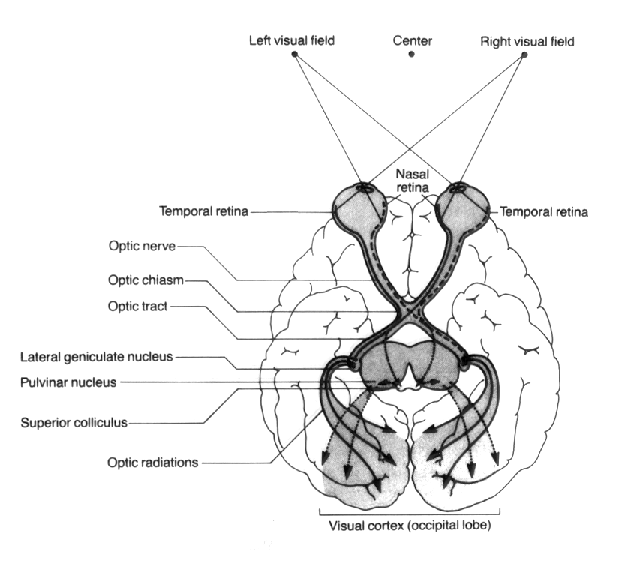
\epsfig{file=pics/sehbahn.eps,width=12cm}
\end{center}
\caption{Skizze der Sehbahn im menschlichen Gehirn von den Augen bis zum
primären visuellen Cortex \protect\citeaffixed{churchland:1992}{aus}.}
\label{sehbahn}
\end{figure}

Am Ende des LGN treten Nervenfasern aus allen Schichten zu einem breiten
Band zusammen, der \emph{Radiatio optica}, das zur Sehrinde aufsteigt.  Die
Sehrinde ist in mehrere abgegrenzete Gebiete, sogenannte \emph{Areale}
unterteilt, die zum Teil sehr spezifische Leistungen (wie z.B.
Bewegungs--, Form-- und Farbsehen) erbringen und in zahlreichen Kanälen
untereinander Information austauschen.  Das außenweltnächste,
\emph{primäre} visuelle Areal (in Affen V1, in Katzen häufig A17 genannt)
ist --- wie die Retina und das LGN --- schichtartig strukturiert.  Im Affen
projiziert das LGN ausschließlich zum primären visuellen Cortex, in
Katzen auch in umliegende Areale.  Auch bei der Projektion vom LGN in den
primären visuellen Cortex fächern die Fasern wieder in geordneter Weise
auf: Die Topologie der Abbildung vom Gesichtsfeld in den Cortex bleibt
somit erhalten.

\begin{figure}[t]
\begin{center}
\begin{minipage}[m]{5cm}
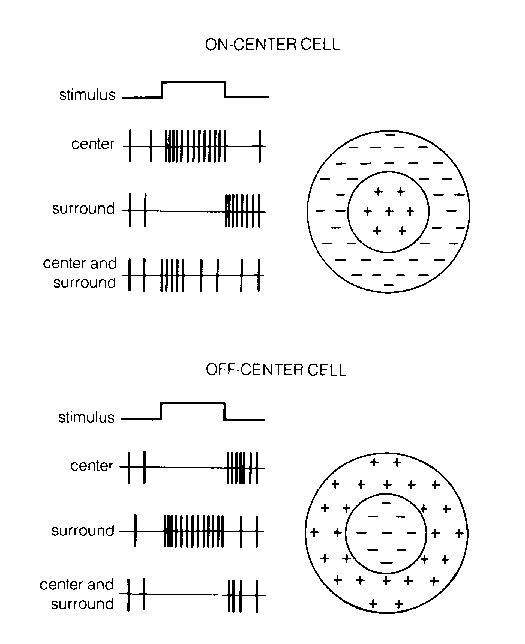
\epsfig{file=pics/rf_onoff.eps,width=5cm}
\end{minipage}
\hskip1cm
\begin{minipage}[m]{6cm}
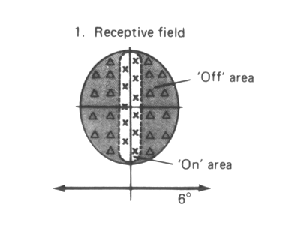
\epsfig{file=pics/rf_simple.eps,width=6cm}
\end{minipage}
\end{center}
\caption{\textbf{a)} Skizze der radialsymmetrischen rezeptiven Felder
sogenannter ``Zentrum--Umfeld--Zellen'' (rechts). Die mit~``$+$''
markierten Gebiete kennzeichnen Bereiche, in denen eine Stimulation zur
Erregung der Zelle führt (``Exzitation''); in den mit~``$-$'' markierten
Bereichen führt eine Stimulation zur Hemmung der Zelle
(``Inhibition''). Nach ihrem Antwortverhalten (skizziert in der linken
Spalte) unterscheidet man 2 Typen: \emph{ON--Zentrum}--Zellen und
\emph{OFF--Zentrum}--Zellen. \textbf{b)} Skizze eines rezeptiven Feldes
einer sog. ``einfachen Zelle''. Ein zentrales, schmales exzitatorisches
Gebiet ist von symmetrischen, inhibitorischen Gebieten umgeben. Der
optimale Stimulus für diese Zelle ist ein vertikal orientierter
Lichtbalken (von $\approx1^\circ\times 8^\circ$ Größe) im Zentrum des
rezeptiven Feldes.}
\label{rfsimple}
\end{figure}

\subsubsection{Rezeptive Felder}
\label{rf}

Bei den Zellen im primären visuellen Cortex stellt man --- wie auch bei
den Ganglienzellen der Retina und den Zellen im LGN --- eine
Spezialisierung auf gewisse Reizmerkmale fest.  Dabei bestimmen in der
Retina zunächst wenige einfache Merkmale, wie z.B.  Position und Größe
eines Reizes, das Antwortverhalten einer Ganglienzelle (jede Zelle im
Zentralnervensystem hat eine Ruheaktivität, die bei geeigneter Stimulation
drastisch erhöht werden kann).  Das Gebiet genau abgegrenzter Position und
Größe auf der Sinnesoberfläche, welches bei Stimulation zur Aktivierung
einer Zelle führt --- also der Verantwortungsbereich dieser Zelle ---
bezeichnet man auch als das \emph{rezeptive Feld} dieser Zelle (siehe
Abb.~\ref{rfsimple}a).  Am Ende der Sehbahn reagieren die Zellen auf immer
abstraktere Merkmale der Außenwelt.  So lassen sich die Zellen im
primären visuellen Cortex oft nur noch mit Lichtreizen einer ganz
bestimmten Position, Größe und Orientierung stimulieren (einfache Zellen,
siehe Abb.~\ref{rfsimple}b).  Eine andere Zellsubpopulation erhöht ihre
Aktivität nur, wenn sich der Stimulus in einer bestimmten Richtung bewegt
(komplexe Zellen).  Zusätzlich sind die Zellen hier spezialisiert auf
Stimuli aus einem bestimmten Auge (man nennt dies ``okulare Dominanz'' der
Zellen).

Etwas verallgemeinernd bezeichnet man oft auch die Menge aller Merkmale,
die ein Reiz besitzen muß, um die Aktivität einer bestimmten Zelle zu
maximieren, als das rezeptive Feld dieser Zelle.  Die Zunahme der
Spezialisierung ist Ausdruck der Konvergenz im visuellen System: entlang
der Sehban erhalten fast alle Zellen Eingänge von mehr als einer anderen,
vorgelagerten Zelle. (Mit dieser anatomischen Beobachtung läßt sich
bereits die Präferenz visueller corticaler Zellen für bestimmte
Stimulusorientierungen erklären; siehe Abb.~\ref{opmodel}.)

\begin{figure}[p]
\begin{center}
\epsfig{file=pics/opmodel.eps,width=9cm}
\end{center}
\caption{Einfaches Model der Orientierungspräferenz \protect\cite{hubel:1962}:
Die Axone mehrerer Zentrum--Umfeld--Zellen konvergieren auf eine einfache
Zelle. Dadurch, daß die rezeptiven Felder der Zentrum--Umfeld--Zellen auf
der Sinnesoberfläche entlang einer Linie angeordnet sind, antwortet die
einfache Zelle selektiv auf Lichtbalken einer bestimmten Orientierung.}
\label{opmodel}
\end{figure}

\begin{figure}[p]
\begin{center}
\begin{minipage}[m]{5.5cm}
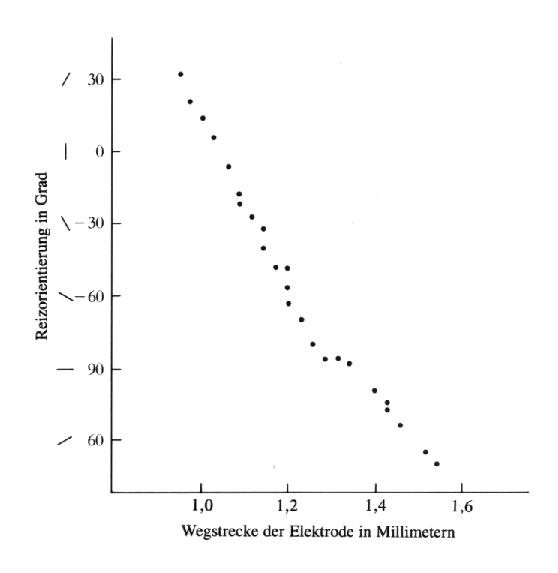
\epsfig{file=pics/opelektrode1.eps,width=5.5cm}
\end{minipage}
\hskip1cm
\begin{minipage}[m]{5.5cm}
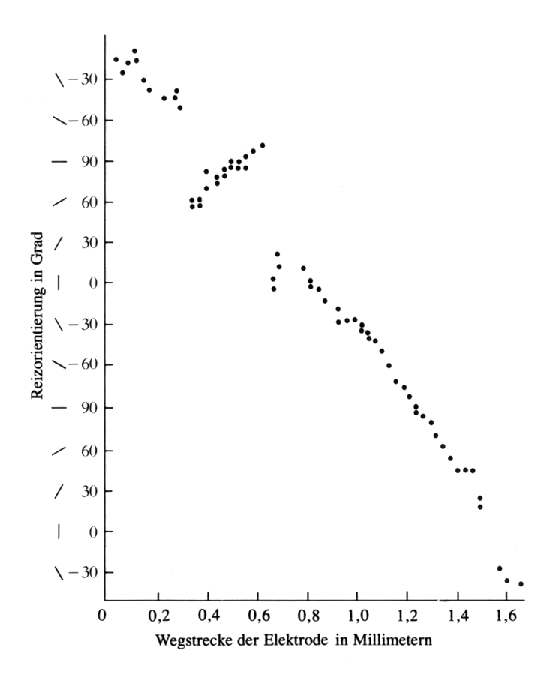
\epsfig{file=pics/opelektrode2.eps,width=5.5cm}
\end{minipage}
\end{center}
\caption{Ergebnis eines typischen Experiments mit tangentialer
Elektrodenführung durch Area 17 in einer Katze für 2 verschiedene
Wegführungen, \protect\citeaffixed{hubel:1989}{aus}.  Aufgetragen ist
jeweils die präferierte Reizorientierung der abgeleiteten Zelle gegenüber
der Entfernung vom Ausgangspunkt der Messung.  \textbf{a)} Die bevorzugte
Reizorientierung ändert sich stetig und linear mit der Wegstrecke.
\textbf{b)} In dieser Messung ändert sich der Drehsinn zweimal sprunghaft
innerhalb einer Strecke von wenigen zehntel Millimetern.}
\label{opelektrode}
\end{figure}

\subsubsection{Kolumnäre Organisation der primären Sehrinde}

Mit einer Mikroelektrode, die schrittweise durch den Cortex geschoben wird,
kann man experimentell den Verlauf der rezeptiven Feldeigenschaften von
Zellen entlang einer Linie im Cortex bestimmen
\citeaffixed{hubel:1989}{siehe z.B.}: Durch die  Mikroelektrode ist
das elektrische Potential einer einzelnen Zelle meßbar.  Das
Aktionspotential einer Zelle im ``Ruhezustand'', also ohne geeignete
Stimulation, überschreitet dabei nur gelegentlich eine kritische Schwelle,
oberhalb der die Zelle einen elektrischen Puls aussendet (die Zelle
``feuert'').  Wird nun ein geeigneter Stimulus auf die Retina projiziert,
so können die Merkmale dieses Stimulus (wie z.B. Größe, Position, usw.)
solange variiert werden, bis die ``Feuerrate'' der betrachteten Zelle
maximiert wurde: das rezeptive Feld der Zelle wurde gefunden.  Auf diese
Weise können innerhalb eines Experiments die rezeptiven Felder mehrerer
Zellen bestimmt werden.

Ein Ergebnis solcher Messungen ist, daß die rezeptiven Feldeigenschaften
untereinanderliegender Zellen identisch sind. Tangential zur
Cortexoberfläche variieren die rezeptiven Feldeigenschaften der Zellen
dagegen i.a. graduell und in gesetzmäßiger Weise mit der Position der
Zellen auf der Cortexoberfläche (vgl. Abb.~\ref{opelektrode}).  Das
primäre visuelle Areal ist somit wie die meisten anderen
sinnesverarbeitenden Bereiche der Hirnrinde \emph{kolumnär} organisiert,
d.h.  Zellen sind zu funktionalen Einheiten (``Kolumnen'') von wenigen
Zehntelmillimetern Durchmesser zusammengefaßt, die sich zylinderförmig
radial in den Cortex erstrecken.

\subsection{Neuronale Karten}

Obwohl die Verschaltung der Retina mit dem primären visuellen Areal, wie
in Abschnitt~\ref{sehbahnkap} dargestellt, über mehrere
``Relaisstationen'' verläuft, bleibt die Topologie der Sinnesoberfläche
unter der Abbildung in den Cortex erhalten, d.h.  benachbarte Neurone im
Cortex haben benachbarte Verantwortungsbereiche im Gesichtsfeld.  Die im
letzten Abschnitt beschriebenen Mikroelektroden--Experimente ließen schon
früh erkennen, daß es sich bei dieser Projektion um eine
zweidimensionale, oftmals stetige Merkmalsabbildung handelt.  Aufgrund der
Nachbarschaftserhaltung läßt sich eine solche Abbildung auch als
\emph{Karte} der Außenwelt ansehen.  Unter einer \emph{neuronalen Karte}
versteht man eine (häufig in Ortskoordinaten) parametrisierte Darstellung
des Verlaufs einer rezeptiven Feldeigenschaft über ein Cortexareal.  Das
naheliegendste Beispiel einer neuronalen Karte ist die sogenannte
\emph{retinotope Karte} im primären visuellen Areal, bei der benachbarte
Neurone auf Reize reagieren, die benachbart im Gesichtsfeld angeordnet sind
(und deshalb benachbart auf die Retina abgebildet werden; dies erklärt das
Attribut ``retinotop'').

Im primären visuellen Cortex sind i.a. auch Karten abstrakterer Merkmale der
\mbox{Außenwelt} angelegt. Diese sind der retinotopen Karte überlagert.
Ein genaueres Bild dieser Karten für ein ausgedehntes Gebiet mit Hilfe von
Mikroelektroden--Experimenten zu erhalten hieße jedoch ``eine
dreidimensionale Frage mit einer eindimensionalen Meßmethode'' zu
beantworten \cite{hubel:1989}.  Mittlerweile gibt es jedoch geeignete
Methoden zur Messung neuronaler Karten. In den folgenden beiden Abschnitten
werden daher die wichtigsten Typen visueller neuronaler Karten zusammen mit
gebräuchlichen Methoden zu ihrer Messung vorgestellt.

\subsubsection{Okulardominanzkarten}
\label{odkarten}

\begin{figure}[t]
\begin{center}
\begin{minipage}[m]{3.9cm}
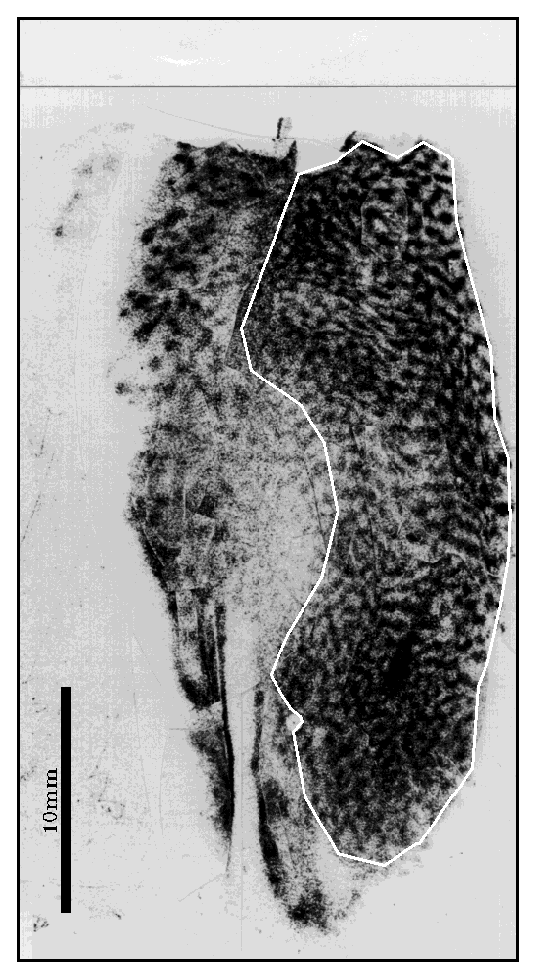
\epsfig{file=pics/normKatze.eps,width=3.9cm,clip=}
\end{minipage}
\hskip2cm
\begin{minipage}[m]{3.9cm}
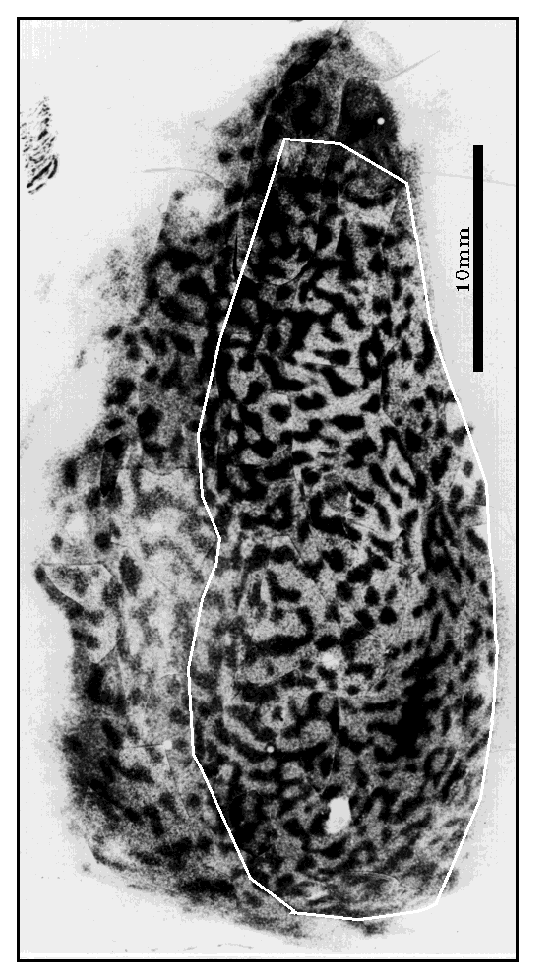
\epsfig{file=pics/strabKatze.eps,width=3.9cm}
\end{minipage}
\end{center}
\caption{Autoradiographie der Okulardominanzkarte aus A17 einer
normalsichtigen (links) und schielenden Katze (rechts)
\protect\citeaffixed{loewel:1987}{neurophysiologische Methode, Karten aus}.}
\label{odsiegrid}
\end{figure}

Neuroanatomische Verfahren zur Visualisierung einer
\emph{Okulardominanzkarte} beruhen auf radioaktiv markierten Stoffen
(typischerweise [$^3$H]--Prolin), die nach Injektion in ein Auge über
axonalen Transport von der Retina in den primären visuellen Cortex
gelangen.  Auf diese Weise reichert sich der radioaktive Marker in den
Zellen an, die in Verbindung mit dem markierten Auge stehen.

Physiologische Messungen solcher Karten verwenden radioaktiv markierte
\mbox{2--deoxyglucose} (2DG), die dem Versuchstier intravenös injiziert
wird. Danach wird ein Auge abgedeckt; der radioaktiv markierte Zucker
reichert sich nun in den Zellen an, die vom geöffneten Auge getrieben
werden. Auf diese Art und Weise läßt sich die funktionale Struktur der
Okulardominanz sichtbar machen.

\setcounter{footnote}{1}
In beiden Experimenten werden anschließend dünne Schnitte des Hirngewebes
angefertigt, die auf Glasplatten ausgefaltet und dann auf einen Film gelegt
werden. Nach langer Belichtung läßt sich anhand einer solchen
\emph{Autoradiographie} die Okularitätskarte als Schwärzungsverteilung
auf dem Film ablesen (siehe Abb.~\ref{odsiegrid}). Man erkennt eine
periodische Struktur, d.h. die schwarzen und weißen Gebiete (also die
Verantwortungsbereiche für markiertes/unmarkiertes bzw. aktives/inaktives
Auge) wechseln sich in bestimmten, regelmäßigen Abständen ab.
Untersuchungen der Wellenlänge\footnote{d.h. der über alle Richtungen
gemittelte Abstand, innerhalb dessen sich die Okulardominanz von einem Auge
zum anderen und wieder zurück verändert} von Okulardominanzkarten aus A17
normalsichtiger Katzen und A17 von Katzen, bei denen früh ein
künstlicher, divergenter Schielwinkel der Augen induziert wurde
(\emph{Strabismus}), zeigen daß die Wellenlänge der
Okulardominanzstruktur bei schielenden Katzen gegenüber der von
normalsichtigen Katzen systematisch erhöht ist \cite{loewel:1994}.
\setcounter{footnote}{1}

\subsubsection{Orientierungskarten}

Zur Messung von \emph{Orientierungskarten} benutzt man heute die
sogenannten \emph{optical imaging}--Verfahren, die Mitte der achtziger
Jahre entwickelt wurden. Diese Verfahren nutzen die veränderten optischen
Eigenschaften aktiver Zellen und ermöglichen dadurch die Sichtbarmachung
der funktionalen Anordung von Zellen unterhalb der Schädeldecke. Die
Veränderungen der optischen Eigenschaften können mit hochempfindlichen
Kameras durch die an einer Stelle geöffnete Schädeldecke des
Versuchstiers abfotographiert werden.  Auf diese Weise erhält man Karten
für beliebige, feste Stimulusmerkmale über ein ausgedehntes Gebiet von
einigen Millimetern Seitenlänge.

Eine der Methoden bedient sich spannungsempfindlicher Farbstoffe, die auf
die Oberfläche des primären visuellen Cortex aufgebracht werden. Das
Versuchstier sieht während des Experiments auf einen Bildschirm, auf dem
z.B. horizontal orientierte Balken durchlaufen. Die Zellen, die am
deutlichsten auf diese Stimulation antworten, äußern dies durch ihre
erhöhte elektrische Aktivität, welche wiederum die optischen
Eigenschaften des Farbstoffes verändert \cite{blasdel:1986,blasdel:1992a}.

Eine bessere Variante dieses Verfahrens ist durch Ausnutzung der
intrinsischen Signale der Cortexschicht nicht auf die langfristig
neurotoxischen, spannungsempfindlichen Farbstoffe angewiesen: Eine erhöhte
Aktivität der Zellen zieht einen erhöhten Blutdurchsatz in ihrer Umgebung
nach sich. Dieser erhöhte Blutdurchsatz äußert sich wiederum in einer
erhöhten Konzentration des Blutfarbstoffes Hämoglobin, der Licht der
Wellenlänge $800nm$ absorbiert. Mit CCD--Kameras kann man die
Intensitätsschwankungen auf der mit $800nm$--Licht beleuchteten
Cortexoberfläche aufnehmen. Die resultierende Hell/Dunkel--Verteilung
spiegelt die Inaktiv/Aktiv--Verteilung im beobachteten Gebiet wieder ---
also die neuronale Karte bezüglich des außen anliegenden Stimulus
\cite{lieke:1989,grinvald:1991}.

Orientierungskarten für eine feste Stimulusorientierung können auch mit
den in Abschnitt~\ref{odkarten} beschriebenen, neurophysiologischen
Methoden erhalten werden.  Der Vorteil des optischen Ableitens im Vergleich
zu neuroanatomischen oder neurophysiologischen Methoden liegt darin, daß
man in solchen Experimenten die neuronalen Karten \emph{in vivo}
erhält. Insbesondere ist man so in der Lage, während eines Experimentes
mehrere Karten für verschiedene Stimulusbedingungen von einem Versuchstier
abzuleiten.

\begin{figure}[t]
\begin{center}
\begin{minipage}{10cm}
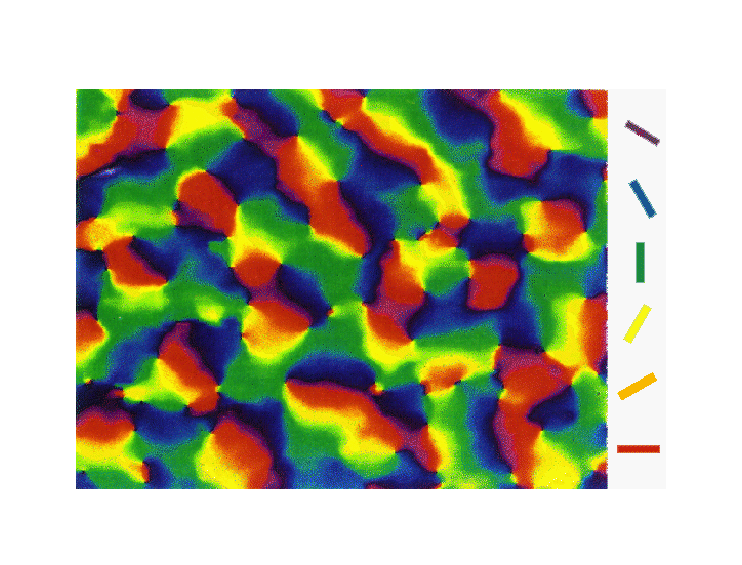
\epsfig{file=pics/OP_affe.eps,width=10cm}
\end{minipage}
\vskip0.5cm
\begin{minipage}[b]{4cm}
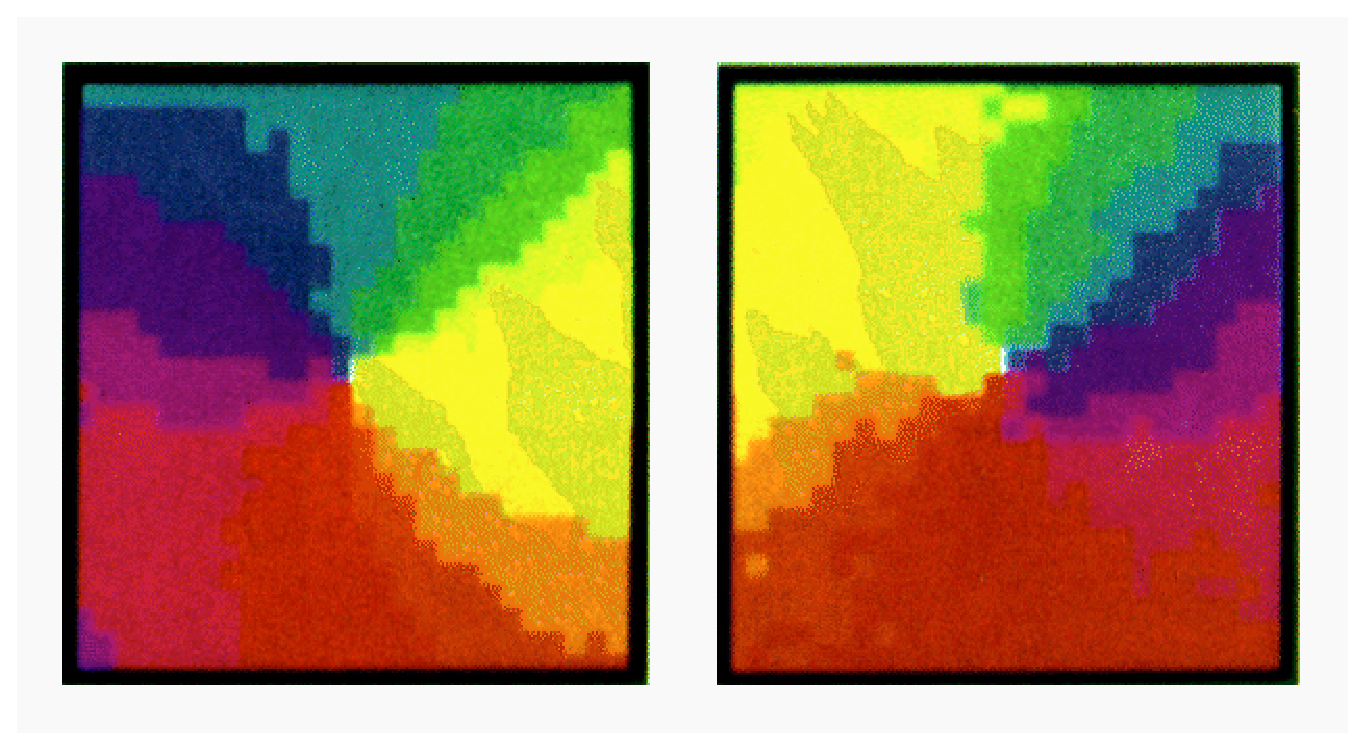
\epsfig{file=pics/pinwheels.eps,width=4cm}
\end{minipage}
\end{center}
\caption{\textbf{Oben:} Karte der Orientierungspräferenz aus dem primären
visuellen Cortex eines Makaken \protect\citeaffixed{blasdel:1992b}{aus}.
\textbf{Unten:} Beispiel für Pinwheels mit Chiralität~\eqref{chi}
$q_i=+\frac{1}{2}$ (links) und $q_i=-\frac{1}{2}$ (rechts). Die
Orientierung ändert sich beim linken Pinwheel im Uhrzeigersinn von gelb
nach rot (d.h. von rechts oblique nach horizontal); beim rechten Pinwheel
verläuft die Orientierungsänderung im Urzeigersinn von rot nach gelb
\protect\citeaffixed{bonhoeffer:1991}{d.h. von horizontal nach rechts
oblique; aus}.}
\label{opblasdel}
\end{figure}

Mehrere, in einem Versuch auf diese Art und Weise gemessenen
Aktivitätsverteilungen (auch ``single--condition'' Karten genannt, siehe
z.B. Abb.~\ref{layout}, rechte Spalte) für jeweils verschiedene
Orientierungen aus dem Intervall $[0^\circ,180^\circ)$ können dann
farblich codiert zu einer Orientierungskarte überlagert werden (siehe
Abb.~\ref{opblasdel}, oben).  Die Orientierungspräferenz als Funktion der
tangentialen Position $\mathbf{x}$ läßt sich folgendermaßen formulieren:

\begin{equation*}
z(\mathbf{x})=\sum\limits_k A_k(\mathbf{x})\; \text{e}^{i2\theta_k}
\label{zfeld}
\end{equation*}

Alle zu den Stimulusorientierungen $\theta_k$ gehörenden
Aktivitätsverteilungen $A_k(\mathbf{x})$ werden hier zu einem komplexen
Feld~$z$ überlagert.  Aus diesem Feld ergibt sich die Orientierungskarte
durch die Relation

\begin{equation*}
\vartheta=\frac{1}{2}\text{arctan}(z).
\end{equation*}

Das auffälligste Srukturelement einer solchen Orientierungskarte sind die
topologischen Punkt--Defekte, in deren Umgebung die
Iso--Orientierungsbereiche wie bei einem Windrad angeordnet sind (sie
werden daher oft auch als \emph{Pinwheels} berzeichnet): In einer
kreisförmigen Umgebung $C_i$ um eine Singularität ändert sich die
Orientierungspräferenz um $\pm 180^\circ$.  Die Positionen $\mathbf{x}_j$
dieser Singularitäten sind dabei die Nullstellen des komplexen Feldes
$z(\mathbf{x})$. Man unterscheidet zwei Sorten solcher Punkt--Defekte nach
ihrer ``Händigkeit'' (vgl. Abb.~\ref{opblasdel}, unten)

\begin{equation}
q_i=\frac{1}{2\pi}\oint_{C_i}\!\!\nabla\vartheta(\mathbf{x})\;ds = \pm
\frac{1}{2}
\label{chi}
\end{equation}

Beide Arten von Singularitäten treten gleich häufig auf.  In allen
natürlichen Karten ändert sich die Orientierungspräferenz bei einem
vollem Umlauf um eine solche Singularität immer nur um $\pm 180^\circ$,
nicht aber um $\pm 360^\circ$ \citeaffixed{penrose:1979}{einen Überblick
über alle theoretisch möglichen Arten solcher Punktdefekte gibt}.

Das nächst charakteristische Element einer Orientierungskarte sind die
sogenannten linearen Zonen. In diesen Gebieten, die etwa 50\% einer
Orientierungskarte ausmachen, laufen die Iso--Orientierungsbereiche
parallel über Strecken von bis zu $1mm$. Die Orientierung zwischen
benachbarten Iso--Orientierungsbereichen verändert sich stetig, d.h. ohne
Sprünge (das Ergebnis eines Mikrolektrodenexperiments, bei dem die
Mikroelektrode senkrecht zur Richtung einer solchen linearen Zone bewegt
wurde, zeigt Abb.~\ref{opelektrode}a).

\subsection{Speziesunterschiede visueller Reizrepräsentationen}
\label{unterschiede}

\begin{figure}[p]
\begin{center}
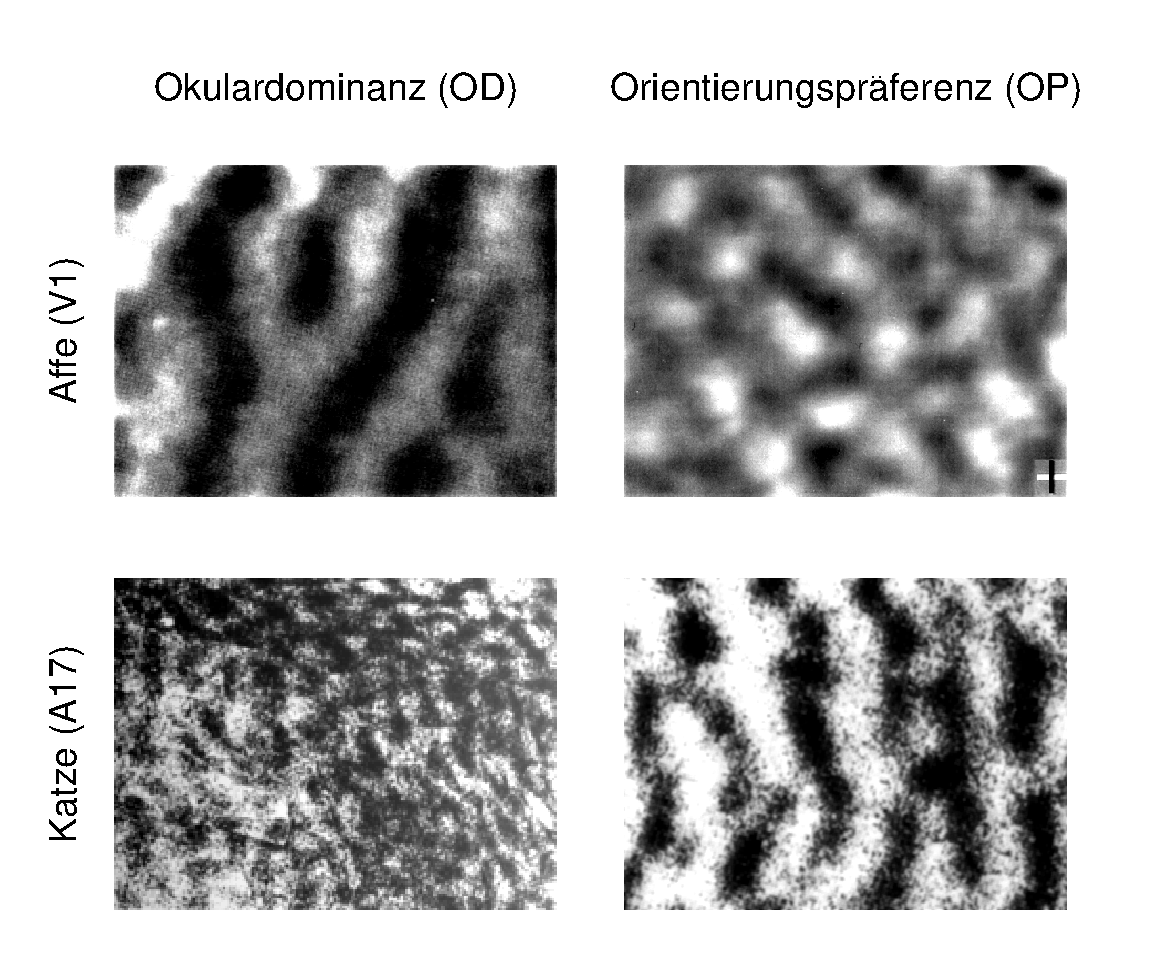
\epsfig{file=pics/monkeycat.eps,width=11cm}
\end{center}
\caption{Layoutvergleich kolumnärer Strukturen aus dem primären visuellen
Cortex von Katzen \protect\citeaffixed{loewel:1987,loewel:1990}{Daten aus} und Affen
\protect\citeaffixed{blasdel:1992a}{Daten aus}.}
\label{layout}
\end{figure}

\begin{figure}[p]
\begin{center}
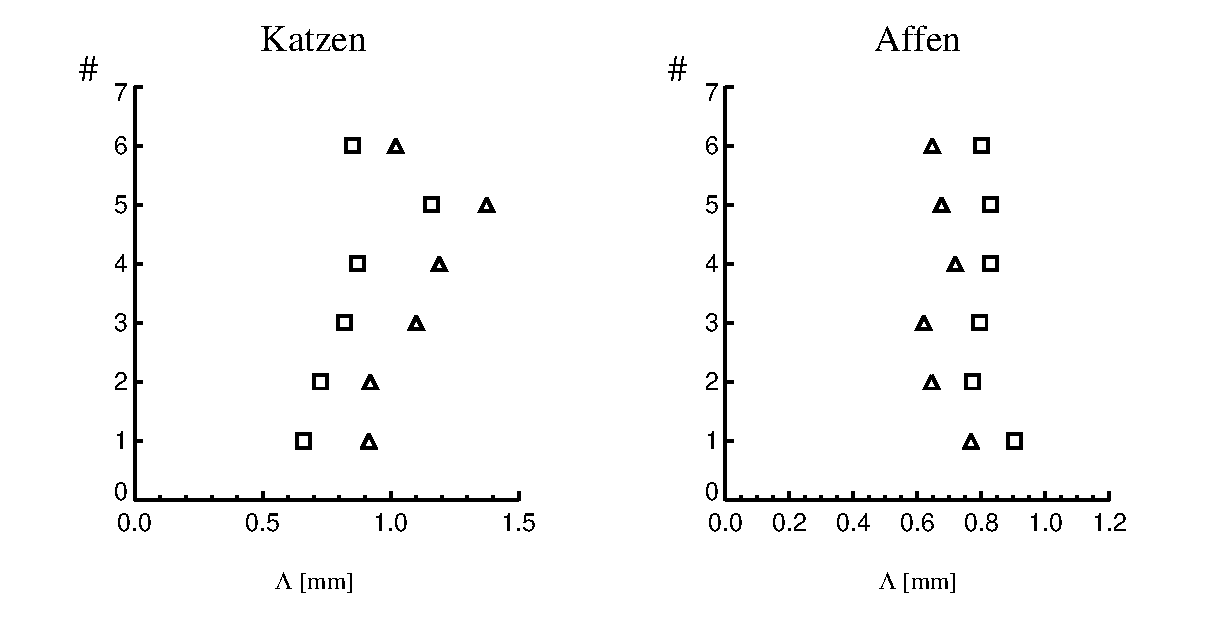
\epsfig{file=pics/wavelength.eps,width=10cm}
\end{center}
\caption{Wellenlängenvergleich typischer Orientierungspräferenz-- und
Okulardominanzkarten aus dem primären visuellen Cortex von Katzen und
Affen. Gezeigt ist das Verhältnis der Wellenlänge der
Orientierungspräferenz~($\triangle$) zur Wellenlänge der
Okuardominanz~($\square$) für mehrere Katzen
\protect\citeaffixed{loewel:1988}{links, Daten aus} und Affen
\protect\citeaffixed{oby:1993b}{rechts, Daten aus}.}
\label{wavelength}
\end{figure}

Vergleicht man nun neuronale Karten aus dem primären visuellen Cortex von
Affen und Katzen, so erkennt man, daß sich sowohl die
Orientierungspräferenz-- (OP) als auch Okulardominanzkarten (OD) in beiden
Spezies unterscheiden. Der erste, auffälligste Unterschied betrifft das
Layout der jeweiligen Karten (siehe Abb~\ref{layout}): Während eine
typische Okulardominanzkarte aus V1 des Affen ein hochreguläres Muster
paralleler Bänder aufzeigt, die senkrecht zu den Arealgrenzen verlaufen
und kaum verzweigen \cite{levayetal:1985,grinvald:1991}, besteht die
typische Okulardominanzkarte aus A17 der Katze aus einem Geflecht perliger,
aneinandergereihter Domänen ohne erkennbare Vorzugsrichtung
\cite{andersonetal:1988,loewel:1987}.  Eine ``single--condition''
Orientierungskarte dagegen, d.h. eine Karte, die für einen Stimulus einer
bestimmten, festen Orientierung erhalten wurde, besteht im Affen aus
perligen, aneinandergereihten Domänen während dieselbe Karte in der Katze
eine streifige Struktur paralleler Bänder aufzeigt.  Berücksichtigt man
nur das Layout, so erscheint eine OD--Karte aus der Katze mit einer
OP--Karte aus dem Affen vergleichbar (und eine OP--Karte aus der Katze mit
einer OD--Karte aus dem Affen siehe dazu Abb.~\ref{layout}).

Ein weiterer Unterschied der Karten in beiden Spezies betrifft die
Wellenlänge~$\Lambda$ der jeweiligen Strukturen
(vgl. Abb~\ref{wavelength}): Ein Vergleich der Wellenlänge der
OD--Struktur mit der Wellenlänge der OP--Struktur aus V1 des Affen ergibt,
daß die mittlere Wellenlänge der OD--Domänen immer größer ist als die
der OP--Domänen.  Das Verhältnis
$\Lambda_{\text{OD}}/\Lambda_{\text{OP}}$ ist ungefähr $6/5$
\cite{oby:1993b}. In der Katze verhält es sich genau umgekehrt: Hier ist
die mittlere Wellenlänge der OP--Struktur immer größer als die der
OD--Struktur; das Verhältnis $\Lambda_{\text{OD}}/\Lambda_{\text{OP}}$
beträgt ungefähr $4/5$ \cite{loewel:1988}.

Okulardominanzkarten aus dem primären visuellen Cortex von Katzen und
Affen unterscheiden sich neben ihrer charakteristischen Wellenlänge um ein
weiteres Merkmal: Der Grad der \emph{Okulardominanzsegregation} --- also
der Grad der Selektivität der Zellen für eines der beiden Augen --- ist
im Affen sowie in der strabismischen und normalsichtigen Katze
unterschiedlich stark ausgeprägt (siehe Abb.~\ref{okuhist}).

\begin{figure}[t]
\begin{center}
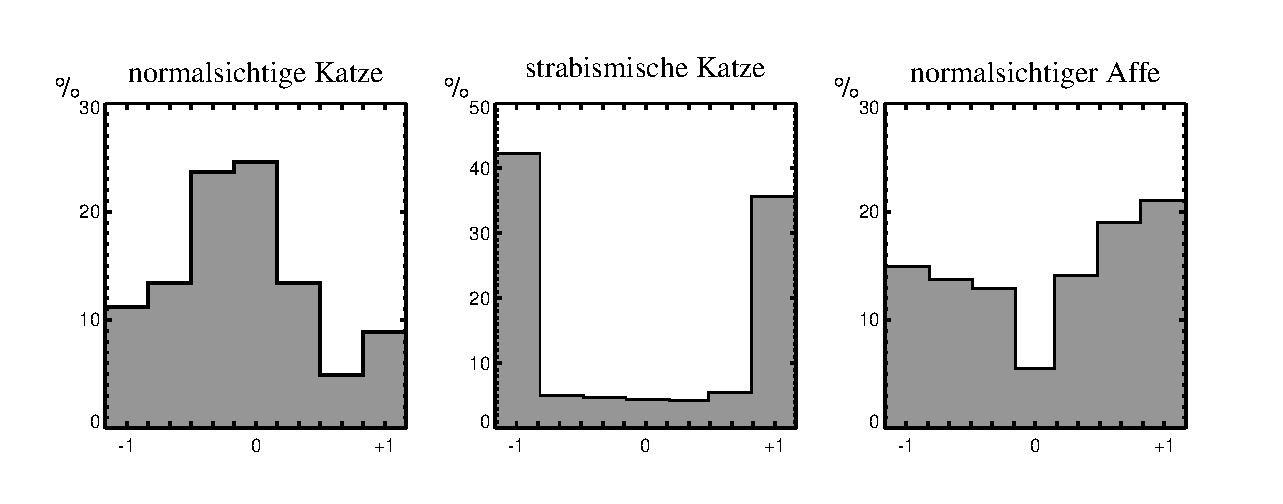
\epsfig{file=pics/okuhist.eps,width=\textwidth}
\end{center}
\caption{Okulardominanzhistogramme für normalsichtige und strabismische
Katzen, sowie für den Affen. Es ist die relative Häufigkeit der Zellen,
die sich entweder nur vom linken ($-1$) oder nur vom rechten ($+1$) oder
von beiden Augen ($0$) stimulieren lassen aufgetragen. Bei normalsichtigen
Katzen sind die meisten Zellen binokular. Bei strabismischen Katzen und
beim Affen überwiegt die Zahl der Zellen, die sich auf eines der beiden
Augen spezialisiert hat \protect\citeaffixed{hubel:1989}{Daten aus}.}
\label{okuhist}
\end{figure}

\subsection[Geometrische Beziehung zwischen
Iso--Orientierungslinien$\ldots$]{Geometrische Beziehung zwischen
Iso--Orientierungslinien und Okulardominanz--Grenzlinien}
\label{90grad}

Untersuchungen von Okulardominanz-- und Orientierungskarten aus V1 des
Makaken ergaben, daß es eine geometrische Beziehung zwischen den Grenzen
der Okulardominanzdomänen und den Iso--Orientierungslinien gibt
\cite{bartfield:1992,oby:1993b}: In allen untersuchten Fällen zeigt die
Statistik ihrer Schnittwinkel einen Trend zu stumpfen Winkeln (siehe
z.B. Abb~\ref{odop_hist}, rechts).

Für die Katze liegt eine solche Untersuchung bislang noch nicht vor, da in
der normalsichtigen Katze der Grad der Okulardominanzsegregation zu schwach
ist, um optisches Ableiten der Okulardominanzkarte zu erlauben (die
Signalstärke ist hier zu gering). Normalerweise wird die
Orientierungskarte in der Katze durch optisches Ableiten, eine
evtl. benötigte Okulardominanzkarte aus dem gleichen Tier jedoch mit
neurophysiologischen Methoden (vgl. Abschn.~\ref{odkarten}) gewonnen. Es
erweist sich dabei insbesondere als schwierig, die beiden auf
unterschiedliche Art und Weise gewonnenen Karten örtlich wieder zur
Deckung zu bringen. Dies wiederum ist natürlich Vorraussetzung, um eine
solche Schnittwinkelstatistik mit einem vertrauenswürdigem Maß an
Genauigkeit erstellen zu können.

\begin{figure}[t]
\begin{center}
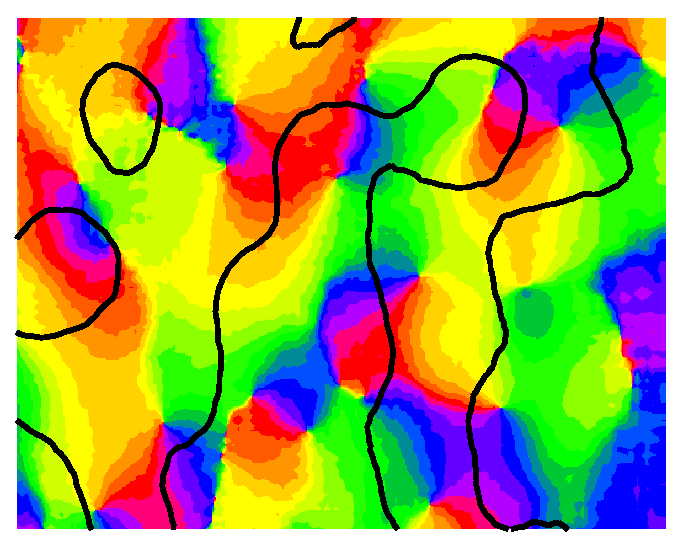
\epsfig{file=pics/odop_pict.eps,width=12.2cm}
\end{center}
\caption{Orientierungskarte aus A17 einer strabismischen Katze. Überlagert
dargestellt (schwarze Linien) sind die Grenzen zwischen den links-- und
rechtsäugigen Domänen der im gleichen Experiment gemessenen
Okulardominanzkarte.}
\label{odop_pict}
\end{figure}

Anhand von Okulardominanz-- und Orientierungskarten aus A17 strabismischer
Katzen, die in Experimenten von Siegrid Löwel am Max--Planck--Institut
für Hirnforschung gemessen wurden, konnte nun erstmals auch für die Katze
eine solche Schnittwinkelstatistik erstellt werden. Bei strabismischen
Katzen ist der Grad der Okulardominanzsegregation sogar stärker als im
Affen (vgl. Abschn.~\ref{unterschiede}, Abb.~\ref{okuhist}), und daher auch
die Okulardominanzkarte durch optisches Ableiten zugänglich. Diese
experimentell gemessenen Karten liegen dabei als Bildmatrix vor (die im
Experiment verwendete CCD--Kamera liefert Bilder mit einer Auflösung von
$128\times 128$ Pixeln). Eine Überlagerung eines Ausschnittes des Bildes
der Orientierungskarte $\theta(\mathbf{x})$ mit dem Bild der Grenzlinien
der Okulardominanzkarte\footnote{Für jede Position $\mathbf{x}$ liegt ein
Wert zwischen $-1$ (linkes Auge) und $+1$ (rechtes Auge) vor. Die
Grenzlinie ist somit definiert als $o(\mathbf{x}) = 0$.} $o(\mathbf{x})$
zeigt Abb.~\ref{odop_pict}. Hier wird schon durch Augenschein wird
deutlich, daß die Grenzen der Okulardominanzdomänen die
Iso--Orientierungsgebiete häufig senkrecht schneiden.
\setcounter{footnote}{1}

Um diesen Zusammenhang zu quantifizieren, benötigt man die Schnittwinkel
zwischen den Iso--Orientierungslinien $\theta(\mathbf{x})=\theta_k$ und den
Okulardominanzgrenzlinien $o(\mathbf{x}) = 0$.  Die Richtung dieser
Konturen ist in jedem Punkt über Drehung der Feldgradienten bestimmbar;
über das Skalarprodukt dieser Gradienten erhält man die Schnittwinkel
$\alpha$ für jeden Punkt $\mathbf{x}$ der Matrix:

\begin{equation*}
\alpha(\mathbf{x})=\text{acos}\!\left(\frac{\pmb\nabla\theta(\mathbf{x})
\;\pmb\nabla o(\mathbf{x})}{\vert\pmb\nabla\theta(\mathbf{x})\;\pmb\nabla
o(\mathbf{x})\vert}\right)
\end{equation*}

Zur Berechnung des räumlichen Gradienten $\pmb\nabla =
{\binom{\partial_1}{\partial_2}}$ auf dem Gitter wurde die diskrete
Approximation
\begin{equation*}
(\pmb\nabla\theta)_{ij}\approx\frac{1}{2\Delta}{\binom{\theta_{i+1,j}\,-\,\theta_{i-1,j}}{\theta_{i,j+1}\,-\,\theta_{i,j-1}}}
\end{equation*}
verwendet (analog für $\pmb\nabla o$). Das Histogramm über die
resultierende Verteilung der Schnittwinkel auf den
Okulardominanzgrenzlinien $\alpha(\left\{\mathbf{x}^\prime\vert\;
o(\mathbf{x}^\prime)=0\right\})$ für den Datensatz in Abb.~\ref{odop_pict}
zeigt Abb.~\ref{odop_hist}, Mitte. In allen vorliegenden Datensätzen aus
insgesamt 7 untersuchten strabismischen Katzen wurde eine solche
$90^\circ$--Statistik der Schnittwinkelverteilung vorgefunden
\citeaffixed{loewel:1996}{siehe}.

Ein wichtiges Phänomen visueller Reizräpresentationen sowohl bei Affen,
als auch wie hier gezeigt bei Katzen, ist demnach die lokale geometrische
Beziehung zwischen den Iso--Orientierungslinien und den Grenzen der
Okulardominanzdomänen: Diese schneiden sich mit überwiegend stumpfen
Winkeln.

\begin{figure}[t]
\begin{center}
\epsfig{file=pics/odop_hist.eps,width=\textwidth}
\end{center}
\caption{Histogramme der Schnittwinkelverteilung zwischen den
Iso--Orien\-tier\-ungs\-linien und den Grenzlinien der Okulardominanzdomänen
im phänomenologischen Modell (siehe Abschn.~\ref{modell}), der
strabismischen Katze \protect\citeaffixed{loewel:1996}{hier für den in
Abb.~\ref{odop_pict} gezeigten Datensatz; weitere siehe} und den Affen
\protect\citeaffixed{oby:1993b}{Daten aus}.}
\label{odop_hist}
\end{figure}

\subsection{Entstehung neuronaler Karten durch Selbstorganisation}
\label{plastizitaet}

Die in den letzten Abschnitten skizzierte, besondere funktionale Anordnung
der Neurone im visuellen Cortex von Katzen und Affen wirft zwei
grundlegende Fragen auf \cite{marlsburg:1973}:

\begin{itemize}
\item Warum sind die Neurone so angeordnet?
\item Durch welche Mechanismen wird die Entstehung und Anordnung dieser
neuronalen Eigenschaften determiniert?
\end{itemize}

In der Diskussion um den Entstehungsmechanismus neuronaler Karten ist dabei
eine immer wiederkehrende Hypothese, daß die diesen Karten
zugrundeliegende Verschaltung der Neurone genetisch prespezifiziert sein
könnte \citeaffixed{wiesel:1974,goedecke:1996}{vgl.}. Die Kodierung der
Struktur solcher Reizrepräsentationen --- die nicht nur im visuellen
Cortex sondern auch in allen anderen Sinnessytemen angelegt sind --- im
Erbgut würde jedoch ein immenses Maß an genetischer Information
benötigen.  Ein weiteres Argument, das diese Hypothese unplausibel
erscheinen läßt, ist die Tatsache, daß mit streng genetisch
determinierten Verschaltungen nicht der im Experiment beobachtete hohe Grad
der \emph{Plastizität} visueller Reizrepräsentationen zu erklären wäre.

Eine Vielzahl von Experimenten belegt jedoch eindrucksvoll, daß die
Struktur --- zumindest aber die Feinstruktur --- visueller
Reizrepräsentationen von der visuellen Erfahrung abhängt. So führt
z.B. der Verschluß eines Auges in einem entwicklungsphysiologisch
kritischem Zeitraum nach der Geburt sowohl bei Katzen als auch bei Affen zu
einer deutlichen Abnahme des Anteils binokularer Neurone. Die meißten
Neurone antworten nach einem gewissen Zeitraum nur noch auf das geöffnete
Auge \citeaffixed{shatz:1978,levay:1980}{siehe z.B.}. Auch die Struktur der
Orientierungskarte ist reizabhängig; jedoch gibt es hierzu aufgrund der
schwierigeren Aufzucht der Tiere nicht dieselbe Fülle an Experimenten wie
für die Okulardominanz. \citeasnoun{blakemore:1970} zogen z.B. Katzen in
einer Umgebung auf, die nur aus horizontalen und vertikalen Reizen bestand:
Der Anteil der auf horizontal/vertikal spezialisierten Neurone
vergrößerte sich dadurch auf Kosten der sonstig orientierten Neurone.

Daß die Anzahl der für einen Sinnesreiz verantwortlichen Neurone mit der
Häufigkeit des Autftretens des Reizes zusammenhängt, ist dabei schon aus
anderen Sinnesbereichen bekannt.  So sind z.B. für die tastsensiblen
Fingerkuppen mehr Neurone verantwortlich als für einen vergleichbar
großen Ausschnitt des Ellenbogenbereichs. Die zahlreichen
Deprivationsexperimente am visuellen System von Katzen und Affen zeigen
deutlich, daß diese Anzahl in einem dynamischen Prozeß an eine
veränderte Reizumgebung angepaßt werden kann.

Die Basis für diese Adaptionsfähigkeit des Gehirns ist dabei nach
heutigem Kenntnistand die Variabilität der Verbindungsstärken zwischen
den Neuronen.  Die Veränderung der Verbindungsstärken findet vorwiegend
an \emph{Synapsen}, den ``Kontaktstellen'' zwischen den Neuronen statt.
Nach einer auf \citeasnoun{hebb:1949} zurückgehenden Vorstellung ändert
sich die Wirksamkeit einer Synapse in Abhängigkeit von der Korrelation
zwischen den Aktivitäten des \emph{präsynaptischen}, d.h. des die Synapse
ansteuernden, und des \emph{postsynaptischen}, d.h. des von der Synapse
angesteuerten Neurons. Diese Vorstellung konnte an einzelnen Synapsen auch
experimentell nachgewiesen werden \cite{brown:1990,kirkwood:1994}.  Die
Hebb'sche Lernregel ermöglicht die Ausrichtung der Architektur des
Nervensystems an die Struktur der Umwelt, wobei wichtige, d.h. häufig
vorkommende Ereignisse, stärker berücksichtigt werden als unwichtige
(seltene). Anhand dieser Lernregel kann das Hirn unüberwacht signifikante
Merkmale aus der Umwelt extrahieren.

Eine viel plausiblere Hypothese für die Entstehung visueller
Reizrepräsentationen ist daher, daß diese ihre Struktur spontan durch
einen Prozeß aktivitätsabhängiger Selbstorganisation ausbilden.  Zum
einen bedarf die Kodierung von Selbstorganisationsregeln im Erbgut --- die
leicht abgewandelt vielleicht auch in anderen Sinnessystemem zur Geltung
kommen könnten --- eines viel geringeren Maßes an genetischer
Information.  Viel wesentlicher ist aber, daß die aktivitätsabhängige
Selbstorganisation einen geeigneten Mechanismus zur Erklärung der
beobachteten Plastizität der Reizrepräsentationen darstellt.
